
\documentclass[nototal,handout]{beamer}
\mode<presentation>
{
  \usetheme{Madrid}
  \setbeamercovered{transparent}
}

\usepackage{verbatim}
\usepackage{fancyvrb}
\usepackage[english]{babel}
\usepackage[latin1]{inputenc}
\usepackage{times}
\usepackage{tikz}
\usepackage[T1]{fontenc}
\usepackage{graphicx} %sjr added
\graphicspath{{figures/}}
\usepackage{hyperref}

\author{Serge Rey}
\institute[sjsrey@gmail.com]{sjsrey@gmail.com}
\title[http://code.google.com/p/otl2latex/]{otl2latex}
\subtitle{User's Guide}
\date[otl2latex]{November 3, 2007}

% Delete this, if you do not want the table of contents to pop up at
% the beginning of each subsection:
\AtBeginSubsection[]
{
  \begin{frame}<beamer>
    \frametitle{Outline}
    \tableofcontents[currentsection,currentsubsection]
  \end{frame}
}


% If you wish to uncover everything in a step-wise fashion, uncomment
% the following command: 
\beamerdefaultoverlayspecification{<+->}
\begin{document}
\begin{frame}
  \titlepage
\end{frame}
\begin{frame}
  \frametitle{Outline}
  \tableofcontents[pausesections]
  % You might wish to add the option [pausesections]
\end{frame}



\section{Introduction} 

\subsection{What is otl2latex?} 

\begin{frame}
	\frametitle{Translator}
 
\begin{block}{otl to tex}
 otl2latex allows you to
 \begin{itemize}
 \item  prepare your document in a powerful outliner
 \item  generate \LaTeX\ markup of your content
 \end{itemize}
 \end{block} \end{frame} 

\subsection{Requirements} 

\begin{frame}
	\frametitle{Operating Systems}
 
\begin{block}{Operating Systems Supported}
 otl2latex has been used successfully on
 \begin{itemize}
 \item  Linux
 \item  Mac OS X
 \item  Windows
 \end{itemize}
 \end{block} \end{frame} 

\begin{frame}
	\frametitle{Software Required}
 
\begin{block}{Packages and Programs}
 \begin{itemize}
 \item  Python http://www.python.org
 \item  \LaTeX
 \item  Beamer http://latex-beamer.sourceforge.net/
 \item  The Vim Outliner http://bike-nomad.com/vim/vimoutliner.html 
 \end{itemize}
 \end{block} \end{frame} 


\section{Usage} 

\subsection{Basics} 

\begin{frame}
	\frametitle{Usage}
 
\begin{block}{From the command line}
  \texttt{python otl2latex.py -p filename.otl filename.tex}
 
 \end{block} 
\begin{block}{Notes}
 \begin{itemize}
 \item  \texttt{filename.tex} will be generated, you don't edit that one.
 \item  You can run all this from withing Vim (see Vim Mappings below).
 \end{itemize}
 \end{block} \end{frame} 

\begin{frame}
	\frametitle{Basics}
 
\begin{block}{Presentations/Beamer}
 \begin{itemize}
 \item  Level 1 in the outline become sections
 \item  Level 2 in the outline become subsections
 \item  Level 3 in the outline become frame titles
 \item  Level 4 in the outline become block titles
 \item  Text in the outline is treated as \LaTeX\ markup
 \end{itemize}
 \end{block} 
\begin{block}{Using Bullets}
  Placing a '*' at the begining of a line will tell otl2latex to begin an itemize list. otl2latex currently supports 3 levels of Itemization.
 \begin{itemize}
 \item  First Level
 \begin{itemize}
 \item  Second Level
 \begin{itemize}
 \item  Third Level
 \end{itemize}
 \item  Second Level
 \end{itemize}
 \end{itemize}
 \end{block} \end{frame} 

\begin{frame}
	\frametitle{Advanced}
 
\begin{block}{Tips}
 \begin{itemize}
 \item  Level 4 can be omitted
 \item  You will have no blocks on that frame
 \end{itemize}
 \end{block} \end{frame} 

\subsection{Vim mappings} 

\begin{frame}
	\frametitle{Vim Mappings: .vimrc}
 
\begin{block}{Processing}
 \begin{itemize}
 \item  ,b will generate a pdf file from your outline
 \item  ,nb will remove all empty lines in your otl file
 \item  ,p will run the current vim buffer through pdflatex
 \end{itemize}
 \end{block} \end{frame} 

\begin{frame}
	\frametitle{Vim Mappings: .vimrc}
 
\begin{block}{Lists}
 \begin{itemize}
 \item  ,i on the first line will create an itemized list of a block of lines
 \item  ,t will mark a block as otl text
 \item  ,I itemize and mark block as otl text
 \end{itemize}
 You need to have a blank line at the end of the block to apply these.
 \end{block} \end{frame} 

\begin{frame}
	\frametitle{Vim Mappings: .vimrc}
 
\begin{block}{Figures}
 \begin{itemize}
 \item ,f (insert mode) will generate stub for figures
 \end{itemize}
 \end{block} \end{frame} 

\begin{frame}
	\frametitle{A figure}
  \begin{center}
 	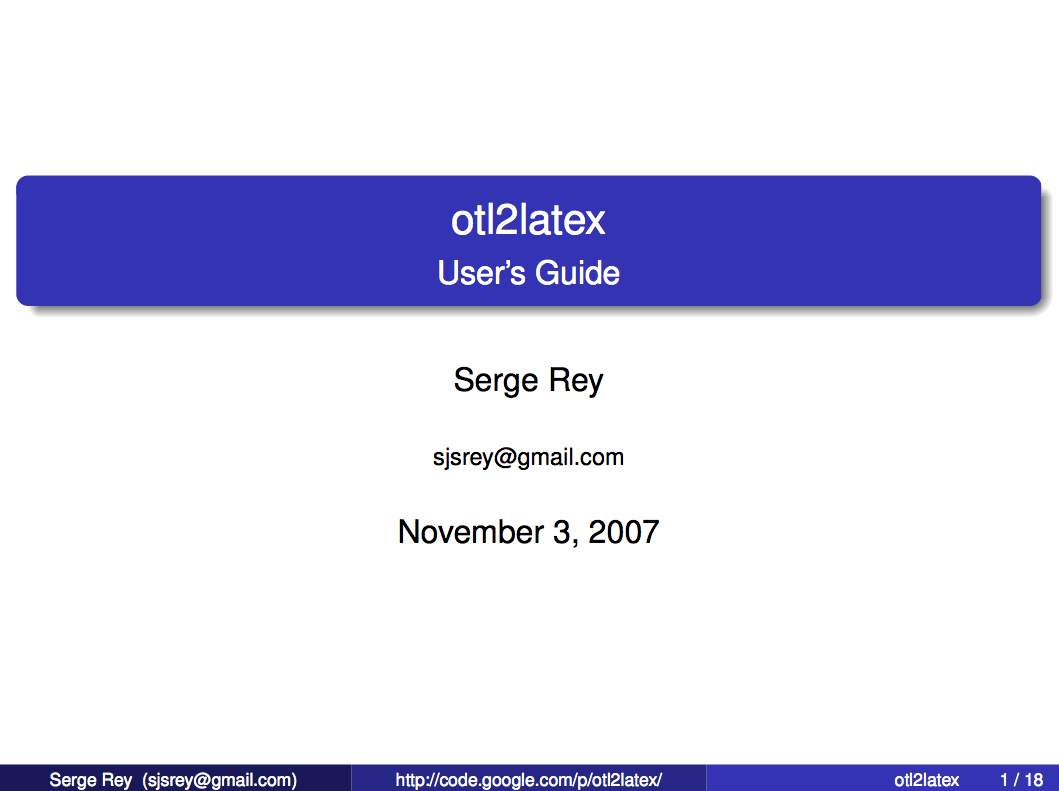
\includegraphics[width=.8\linewidth]{otl2latex.png}
   \end{center}
 \end{frame} 

\begin{frame}
	\frametitle{A figure}
 \begin{center}
 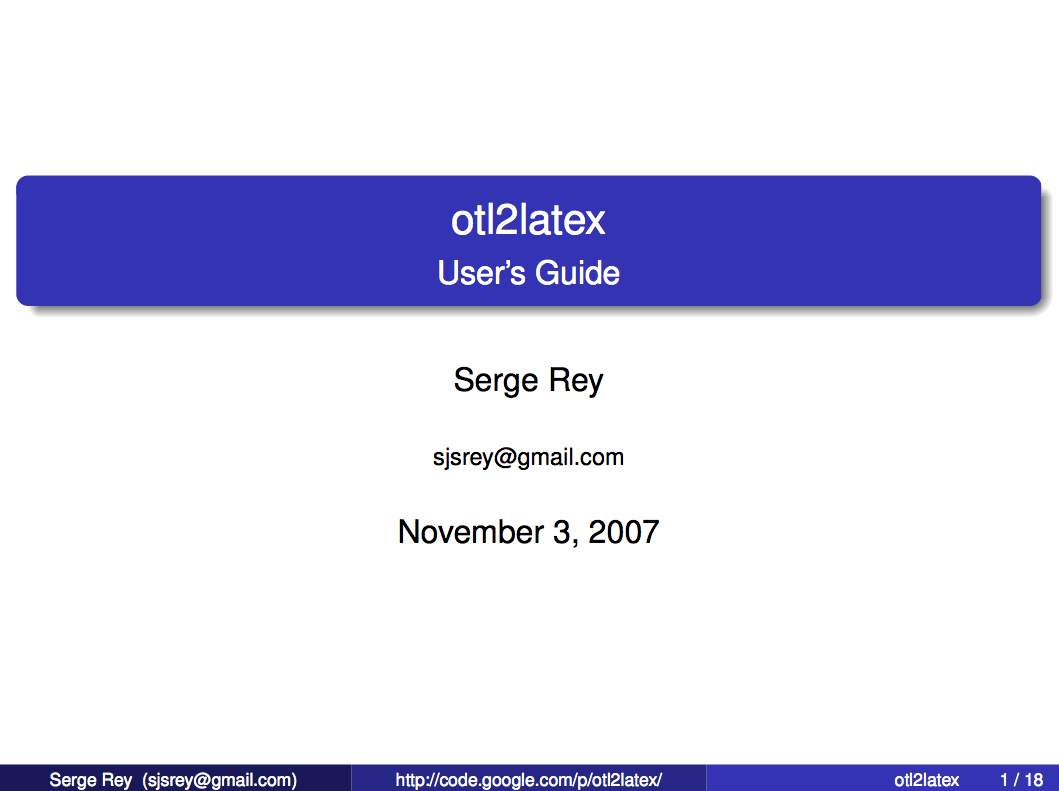
\includegraphics[width=.8\linewidth]{otl2latex.png}
 \end{center}
 \end{frame} 

\subsection{Future Extensions} 

\begin{frame}
	\frametitle{Move to vim script}
 
\begin{block}{.vimrc to otl2latex.vim}
 \begin{itemize}
 \item Currently we are just embedding mappings in .vimrc
 \item Ok for testing, not very polished for end user
 \end{itemize}
 \end{block} \end{frame} 

\begin{frame}
	\frametitle{Reverse Engineering}
 
\begin{block}{latex2otl}
 \begin{itemize}
 \item take a tex file
 \item generate the otl file
 \end{itemize}
 \end{block} \end{frame} 


\section{} 


\section{}
\end{document}
